%Ne pas numéroter cette partie
\part*{Annexes}
%Rajouter la ligne "Annexes" dans le sommaire
\addcontentsline{toc}{part}{Annexes}

\addtocontents{toc}{\protect\setcounter{tocdepth}{0}}

\appendix
\section{Tableaux des différences finies}
Pour la méthode  différences finies, on a utilisé les tableaux suivants pour les schémas des différents ordres, tirés de "Méthodes Numériques, Équations aux Dérivées Partielles (EDP)" de l'institut d'optique Paritech.

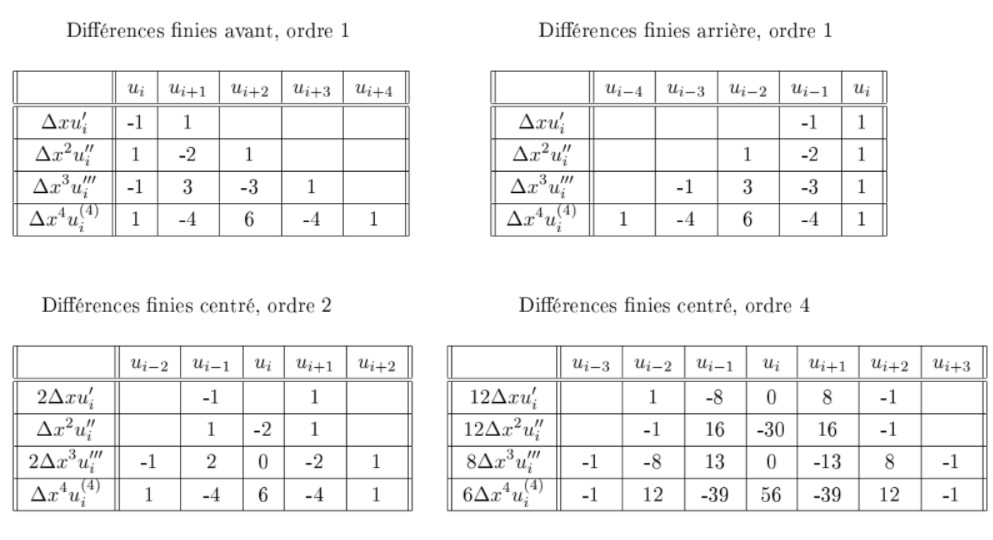
\includegraphics[width=1\textwidth]{./annex1}~\\[1cm]

\section{Solutions pour la partie comparaison}
\begin{figure}[H]
\begin{minipage}[b]{.46\linewidth}
\centering\epsfig{figure=exact.png,width=\linewidth}
\caption{Solution exacte
    \label{fig1}
    }
\end{minipage} \hfill
\begin{minipage}[b]{.46\linewidth}
\centering\epsfig{figure=explicite.png,width=\linewidth}
\caption{Euler explicite\label{fig2}}
\end{minipage}
\end{figure}

\begin{figure}[H]
\begin{minipage}[b]{.46\linewidth}
\centering\epsfig{figure=implicite.png,width=\linewidth}
\caption{Euler implicite\label{fig1}}
\end{minipage} \hfill
\begin{minipage}[b]{.46\linewidth}
\centering\epsfig{figure=RK.png,width=\linewidth}
\caption{Runge-Kutta \label{fig2}}
\end{minipage}
\end{figure}